
\chapter{Analysis}

\section{Introduction}

\subsection{Client Identification}
My client, Shahida Rahman, is an Author, and the Director and Secretary of Perfect Publishers Ltd, which has been a self publishing company since 2005. This means that the author pays Perfect Publishers to publish their book.
 She published her first book through Perfect Publishers Ltd, and this was when the company was born. She is 42 years old and is a mother of 4 children. Shahida uses computers to deal with online enquiries and to publish books from all over the world. Furthermore, she also produces the royalty statements for each book twice yearly. Aside from this, she has little experience with computers. Shahida generally uses a computer for research, social networking and reading the news. Every book is outsourced to an Editor and a Cover Designer. When the book is fully edited and formatted to the right specifications, they return the ready to print files to Shahida, who sends the books off to print. They track the books and their details manually using a database on an Excel Spreadsheet. Currently, it is difficult to keep all the data up to date and it is rather disorganised. Shahida would like to be able to look up a book/number of books in the system by using the details, such as the Author/Title/Date etc. She would also like the new system to link this database with information about the royalties of each book, and when they are needed to be paid every six months. The system could send an email to her, updating her about these. Shahida also wants the system to be able calculate the royalties by using the details given by the user.

\subsection{Define the current system}
The system that is currently being used consists of Shahida entering the book and its details into the spreadsheet. These details are taken from the enquiries that she receives via email, and include; author, book title, size, number of pages, hardback/paperback, mat or gloss, crème or white paper, font and font size. She also records their details in a separate spreadsheet, which includes their email, phone number, and address. Subsequently, Shahida waits for full payment and then sends the customer an invoice. She then contacts her editor and her illustrator to start work on the book. Shahida refers to her company's website, where the calculated prices are ready for books, in order to correctly price the book, in accordance to the book’s details. Once the book is finished, the book is sent off to print, and the author receives 25 copies.

\subsection{Describe the problems}
There are numerous problems with the current system. First of all, the usage of the spreadsheet makes it harder to find a customer and their details, and their book’s details. This is because the spreadsheet is much disorganised. Furthermore, it is harder to keep track of the details of each book, meaning it is difficult to update the details of the book when necessary. Also, if the same author makes an enquiry about another book, her details must be entered into the spreadsheet again, which could cause inconsistencies in the data, because for instance, the customer may move house, meaning their address would need changing, and it would be difficult to find and update all entries where their address is recorded.

\subsection{Section appendix}
\begin{figure}[H]
    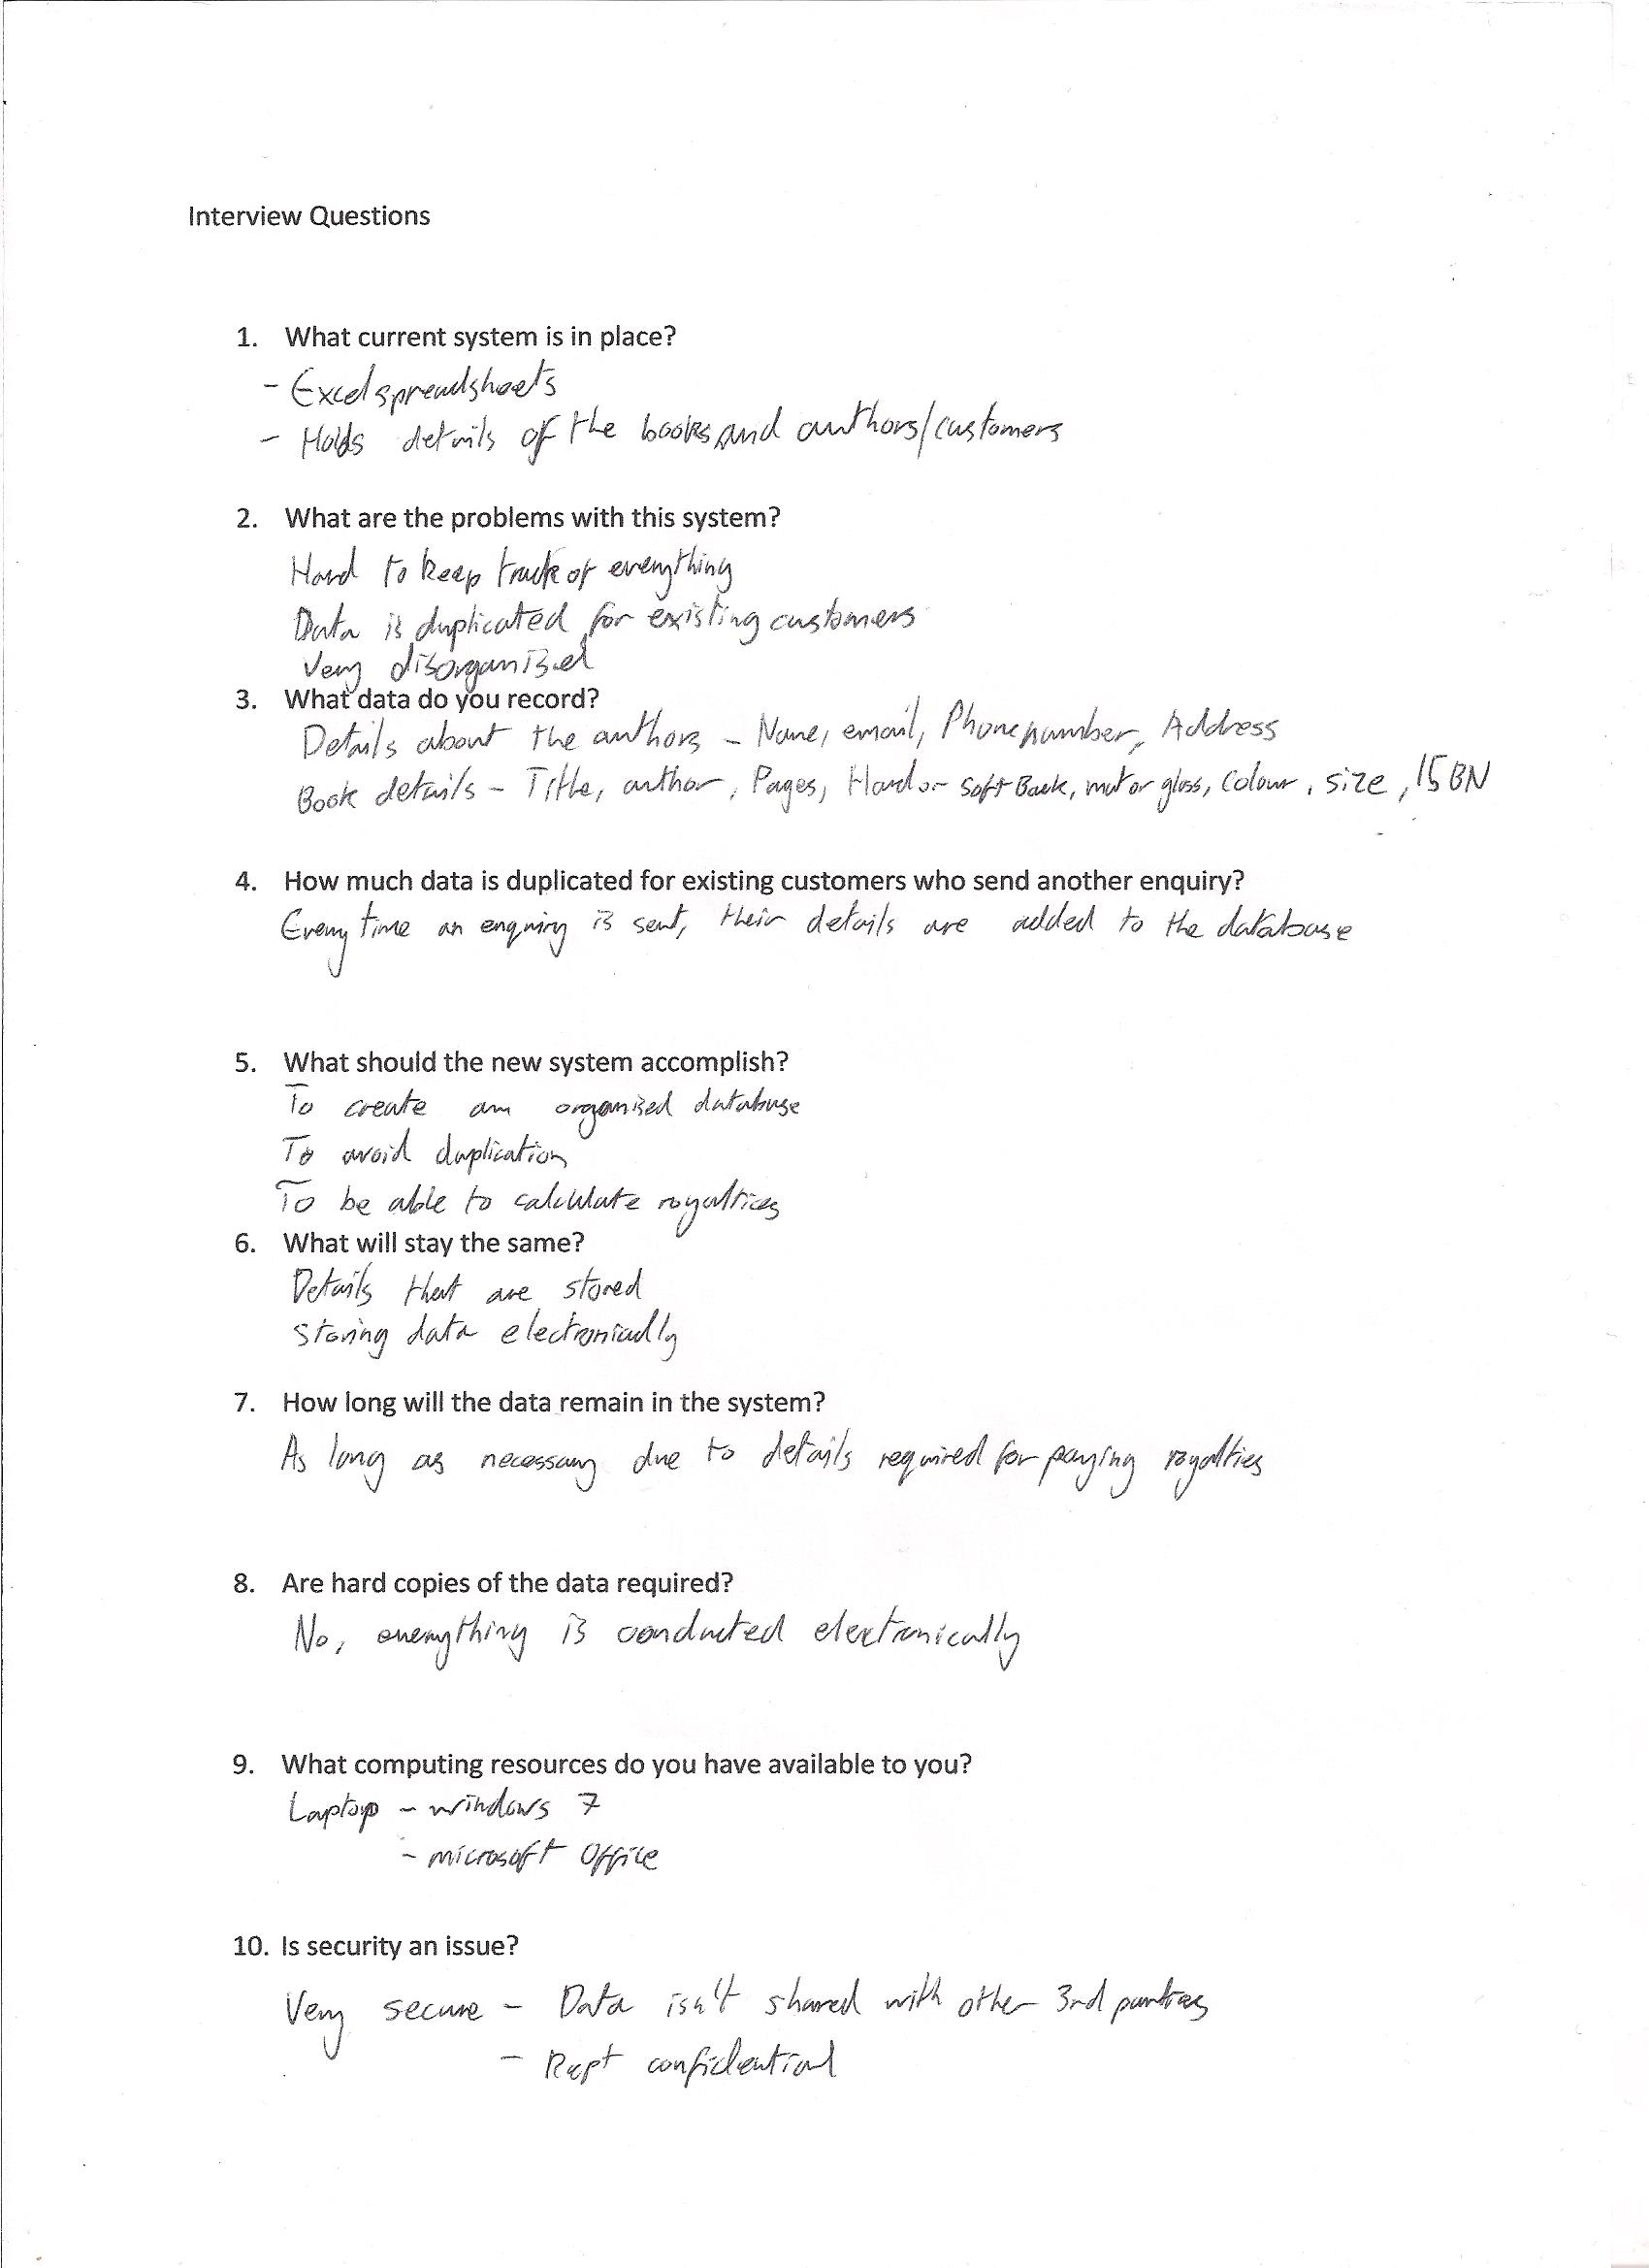
\includegraphics[width=\textwidth]{./Analysis/Interview Questions 1.jpg}
\end{figure}

\begin{figure}[H]
    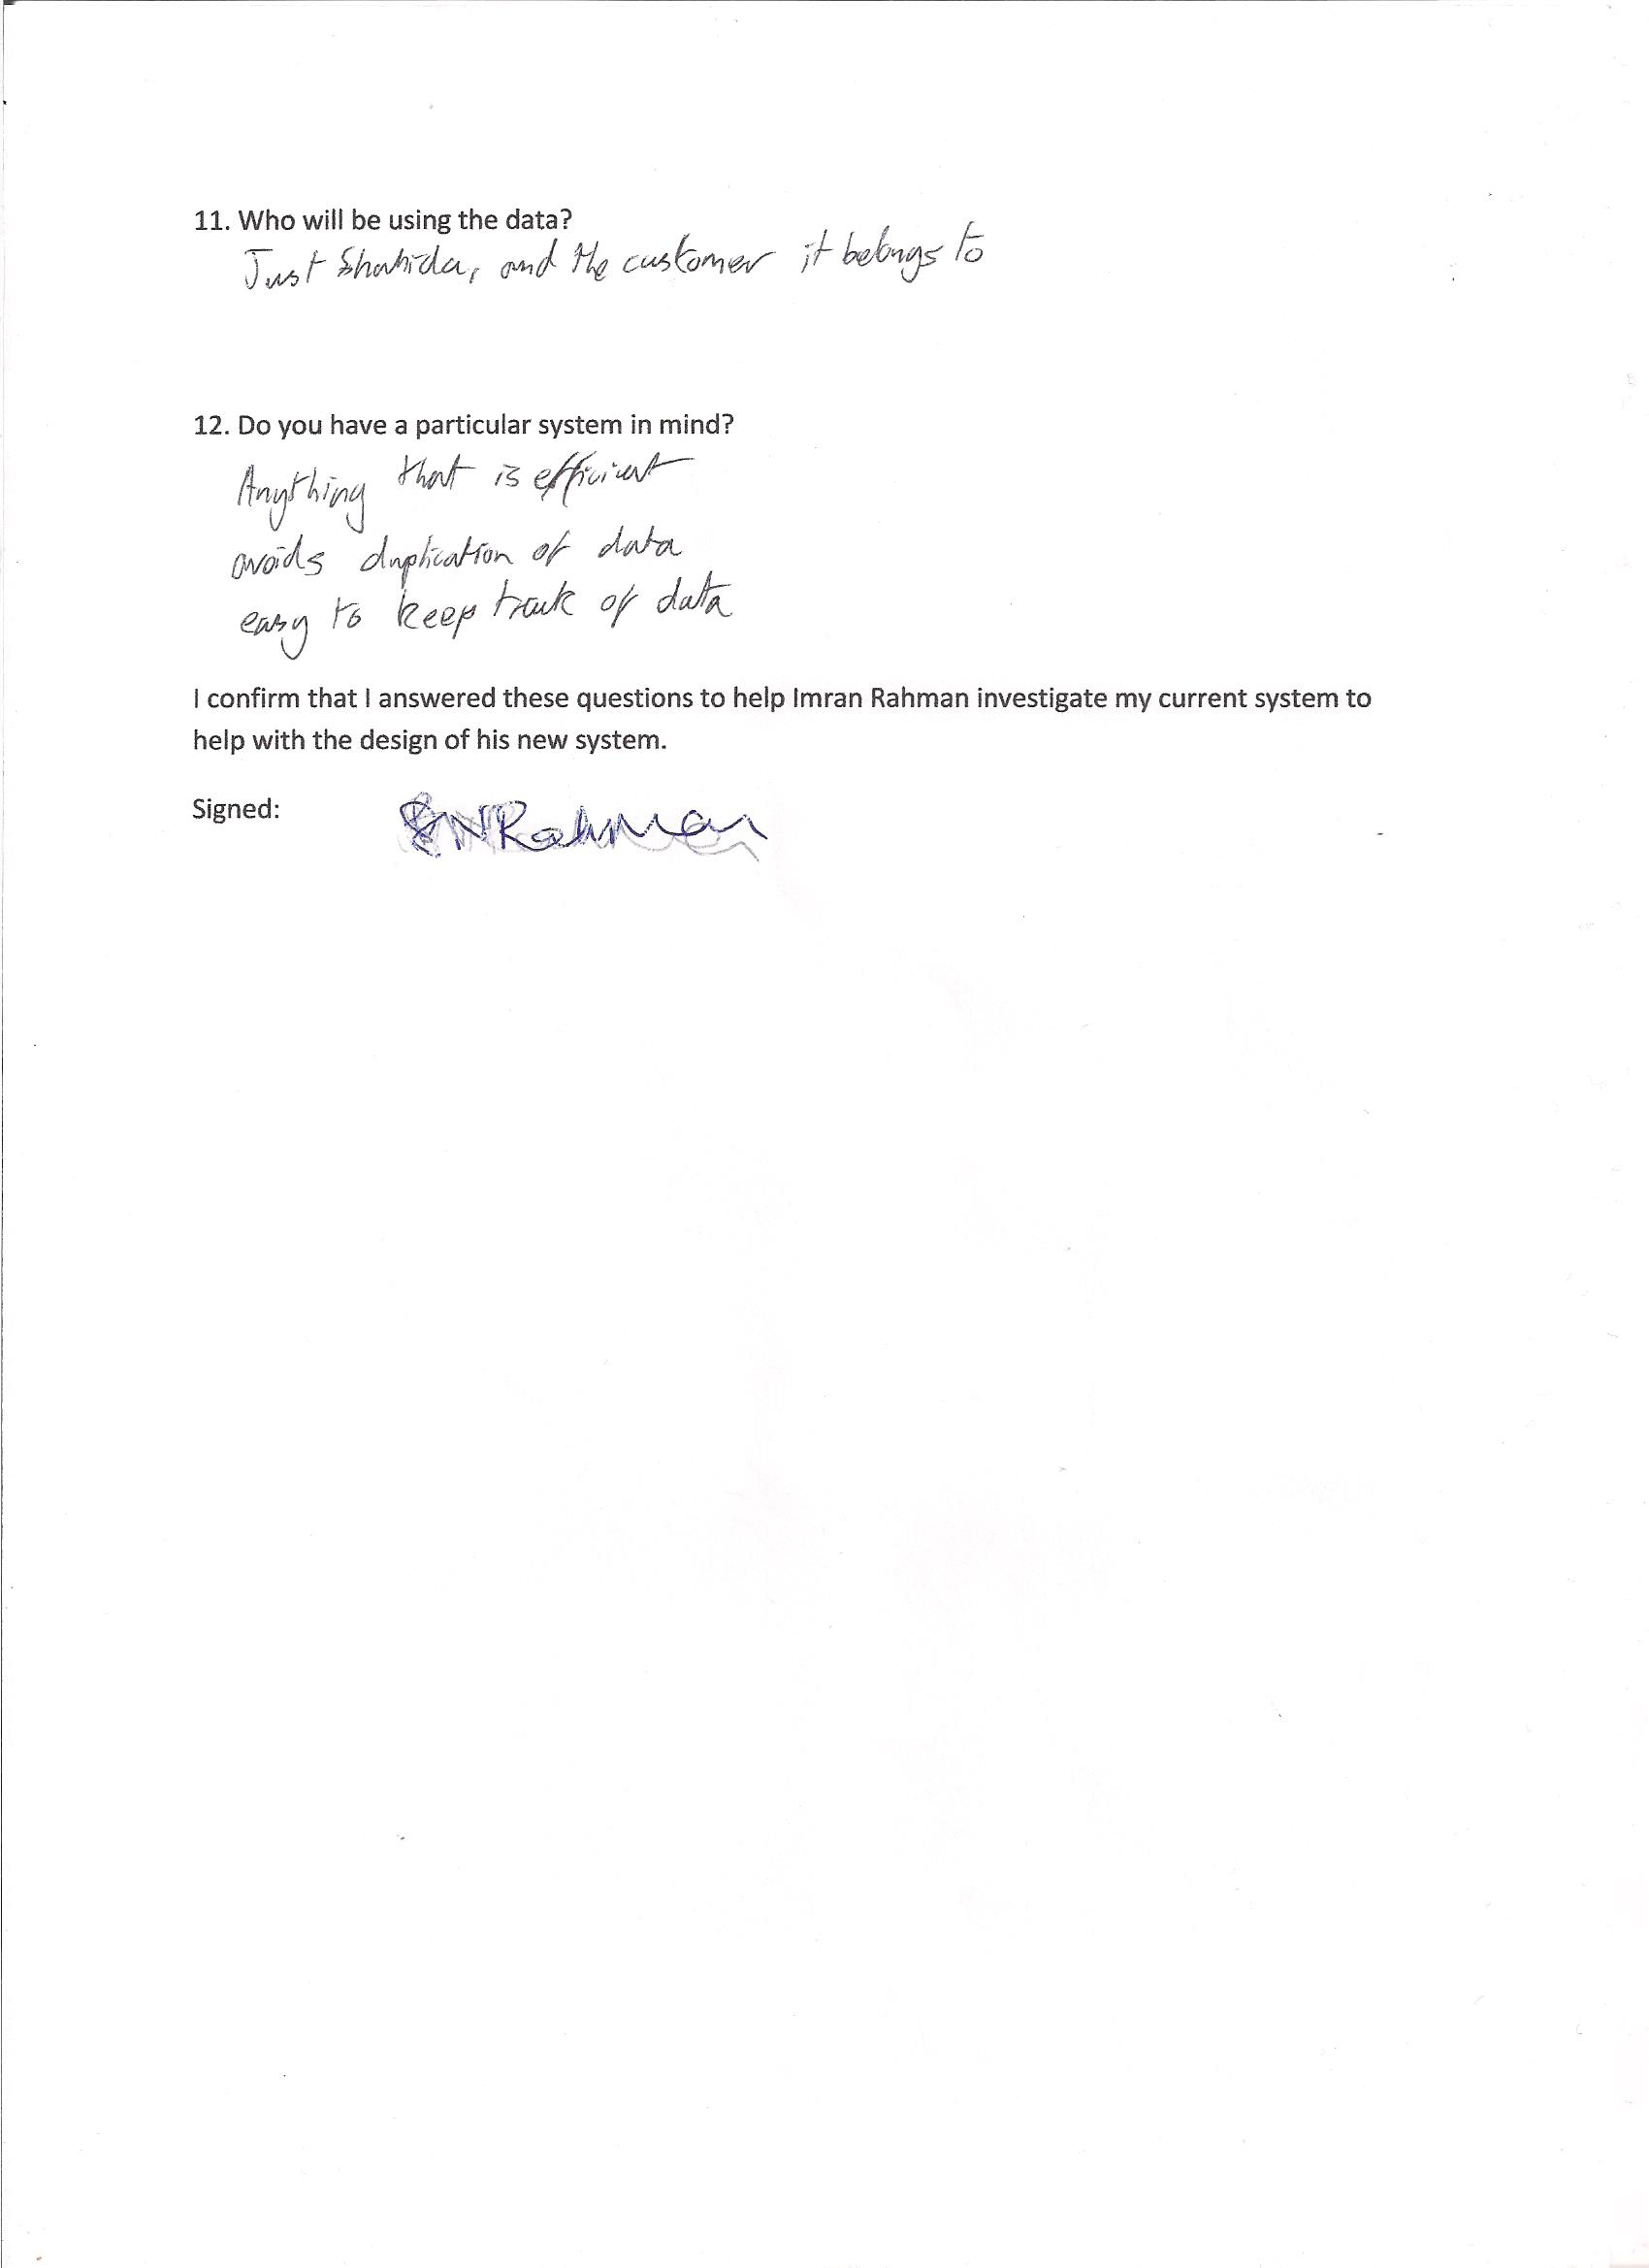
\includegraphics[width=\textwidth]{./Analysis/Interview Questions 2.jpg}
\end{figure}

\section{Investigation}

\subsection{The current system}

\subsubsection{Data sources and destinations}
In the current system there are three key data sources that are used. These are Shahida herself, the customer and the spreadsheets. The Customer sends the enquiry, which holds all the necessary information, and this is sent via email. The details of the book are stored in one spreadsheet, and the person details of the customer are stored in a seperate spreadsheet, linked to the details of the book. These details are agreed seperately from the enquiry, between Shahida and the customer. Details such as the book size, page number, hardback/softback and paper type are used to calculate the cost for the customer, which is used to create an invoice which is sent to the customer. This is the first output of the system. A copy of every invoice is stored on Shahida's computer. Once Shahida receives full payment, the work is conducted and completed. If the customer wishes to publish another book, they send another enquiry, and their personal data is duplicated because of the details of the new book which are added. Every six months after the book has been published, the royalties must be paid to the author. The royalties are the profit that the author makes from sales of her book frm bookshops.



\begin{center}
\begin{tabular}{|p{2.5cm}|p{3.5cm}|p{3.5cm}|p{2.5cm}|}
    \hline
    \textbf{Source} & \textbf{Data} & \textbf{Example Data} & \textbf{Destination} \\ \hline
    \pythoninline{Customer Enquiry} & \pythoninline{Forename} & \pythoninline{Peter} & \pythoninline{Shahida}  \\ \hline
    \pythoninline{Customer Enquiry} & \pythoninline{Surname} & \pythoninline{Parker} & \pythoninline{Shahida}  \\ \hline
    \pythoninline{Customer Enquiry} & \pythoninline{Email} & \pythoninline{mail@example.com} & \pythoninline{Shahida}  \\ \hline
    \pythoninline{Customer} & \pythoninline{Address} & \pythoninline{1 Example Road} & \pythoninline{Shahida}  \\ \hline
    \pythoninline{Customer} & \pythoninline{Postcode} & \pythoninline{AB1 2CD} & \pythoninline{Shahida}  \\ \hline
    \pythoninline{Customer} & \pythoninline{Phone Number} & \pythoninline{07123456789} & \pythoninline{Shahida}  \\ \hline
    \pythoninline{Shahida} & \pythoninline{Forename} & \pythoninline{Peter} & \pythoninline{Database}  \\ \hline
    \pythoninline{Shahida} & \pythoninline{Surname} & \pythoninline{Parker} & \pythoninline{Database}  \\ \hline
    \pythoninline{Shahida} & \pythoninline{Email} & \pythoninline{mail@example.com} & \pythoninline{Database}  \\ \hline
    \pythoninline{Shahida} & \pythoninline{Address} & \pythoninline{1 Example Road} & \pythoninline{Database}  \\ \hline
    \pythoninline{Shahida} & \pythoninline{Postcode} & \pythoninline{AB1 2CD} & \pythoninline{Database}  \\ \hline
    \pythoninline{Shahida} & \pythoninline{PhoneNumber} & \pythoninline{07123456789} & \pythoninline{Database}  \\ \hline
    \pythoninline{Shahida} & \pythoninline{Invoice} & \pythoninline{-} & \pythoninline{Customer}  \\ \hline
    \pythoninline{Customer} & \pythoninline{Payment} & \pythoninline{£1000} & \pythoninline{Shahida}  \\ \hline
    \pythoninline{Shahida} & \pythoninline{Cover Preferences} & \pythoninline{-} & \pythoninline{Cover Designer}\\ \hline
    \pythoninline{Shahida} & \pythoninline{Book} & \pythoninline{-} & \pythoninline{Editor}  \\ \hline
    \pythoninline{Editor} & \pythoninline{Completed Book} & \pythoninline{-} & \pythoninline{Shahida}  \\ \hline
    \pythoninline{Cover Designer} & \pythoninline{Completed Cover} & \pythoninline{-} & \pythoninline{Shahida} \\ \hline
    \hline
\end{tabular}
\end{center}


\subsubsection{Algorithms}
In the current system there are four Algorithms which are being used. The first sends an invoice to the customer and checks whether Shahida has recieved full payment. Once Shahida has received full payment, she, her cover designer and her editor can begin working on the book. The second algorithm checks whether the work has been completed, so that the completed book can then be sent off for printing. The third calculates the royalties which are paid every six months to the author.

\begin{algorithm}[H]
    \caption{First Algorithm - Sending an invoice and Checking for Payment}
\begin{algorithmic}[1]
\SET{$InvoiceSent$}{$false$}
\SET{$Payment$}{$false$}
\State

\While{$InvoiceSent = false$}

    Check Website for Price

    Create Invoice

    Send Invoice

    \SET{$InvoiceSent$}{$true$}

\EndWhile

\While{$Payment = false$}

     Check For Payment

     \If{$Payment Received$}

     	Payment = true

     \EndIf
\EndWhile
\end{algorithmic}
\end{algorithm}


\begin{algorithm}[H]
    \caption{Second Algorithm - Checking If Work is Completed}
\begin{algorithmic}[1]
\SET{$WorkComplete$}{$false$}
\SET{$CoverComplete$}{$false$}
\SET{$BookComplete$}{$false$}
\State

\While{$WorkComplete = false$}
    
    Get Completed Cover from Cover Designer

    \SET{$CoverComplete$}{$true$}

    Get Completed Book from Editor

    \SET{$BookComplete$}{$true$}

    \If{$BookComplete \ and \ CoverComplete$}

        \SET{$finished$}{$true$}

    \EndIf
\EndWhile
\end{algorithmic}
\end{algorithm}

\begin{algorithm}[H]
    \caption{Third Algorithm - Calculating the Royalties}
\begin{algorithmic}[1]
\SEND{$"Enter\ the\ wholesale\ price."$}
\RECEIVE{$wholesaleprice$}
\SEND{$"Enter\ the\ quantity."$}
\RECEIVE{$quantity$}
\SEND{$"Enter\ the\ print\ cost."$}
\RECEIVE{$printcost$}

\SET{$royalties$}{$(quantity\ *\ wholesale)\ -\ printcost$} 

\end{algorithmic}
\end{algorithm}

\subsubsection{Data flow diagrams}

\begin{figure}[H]
    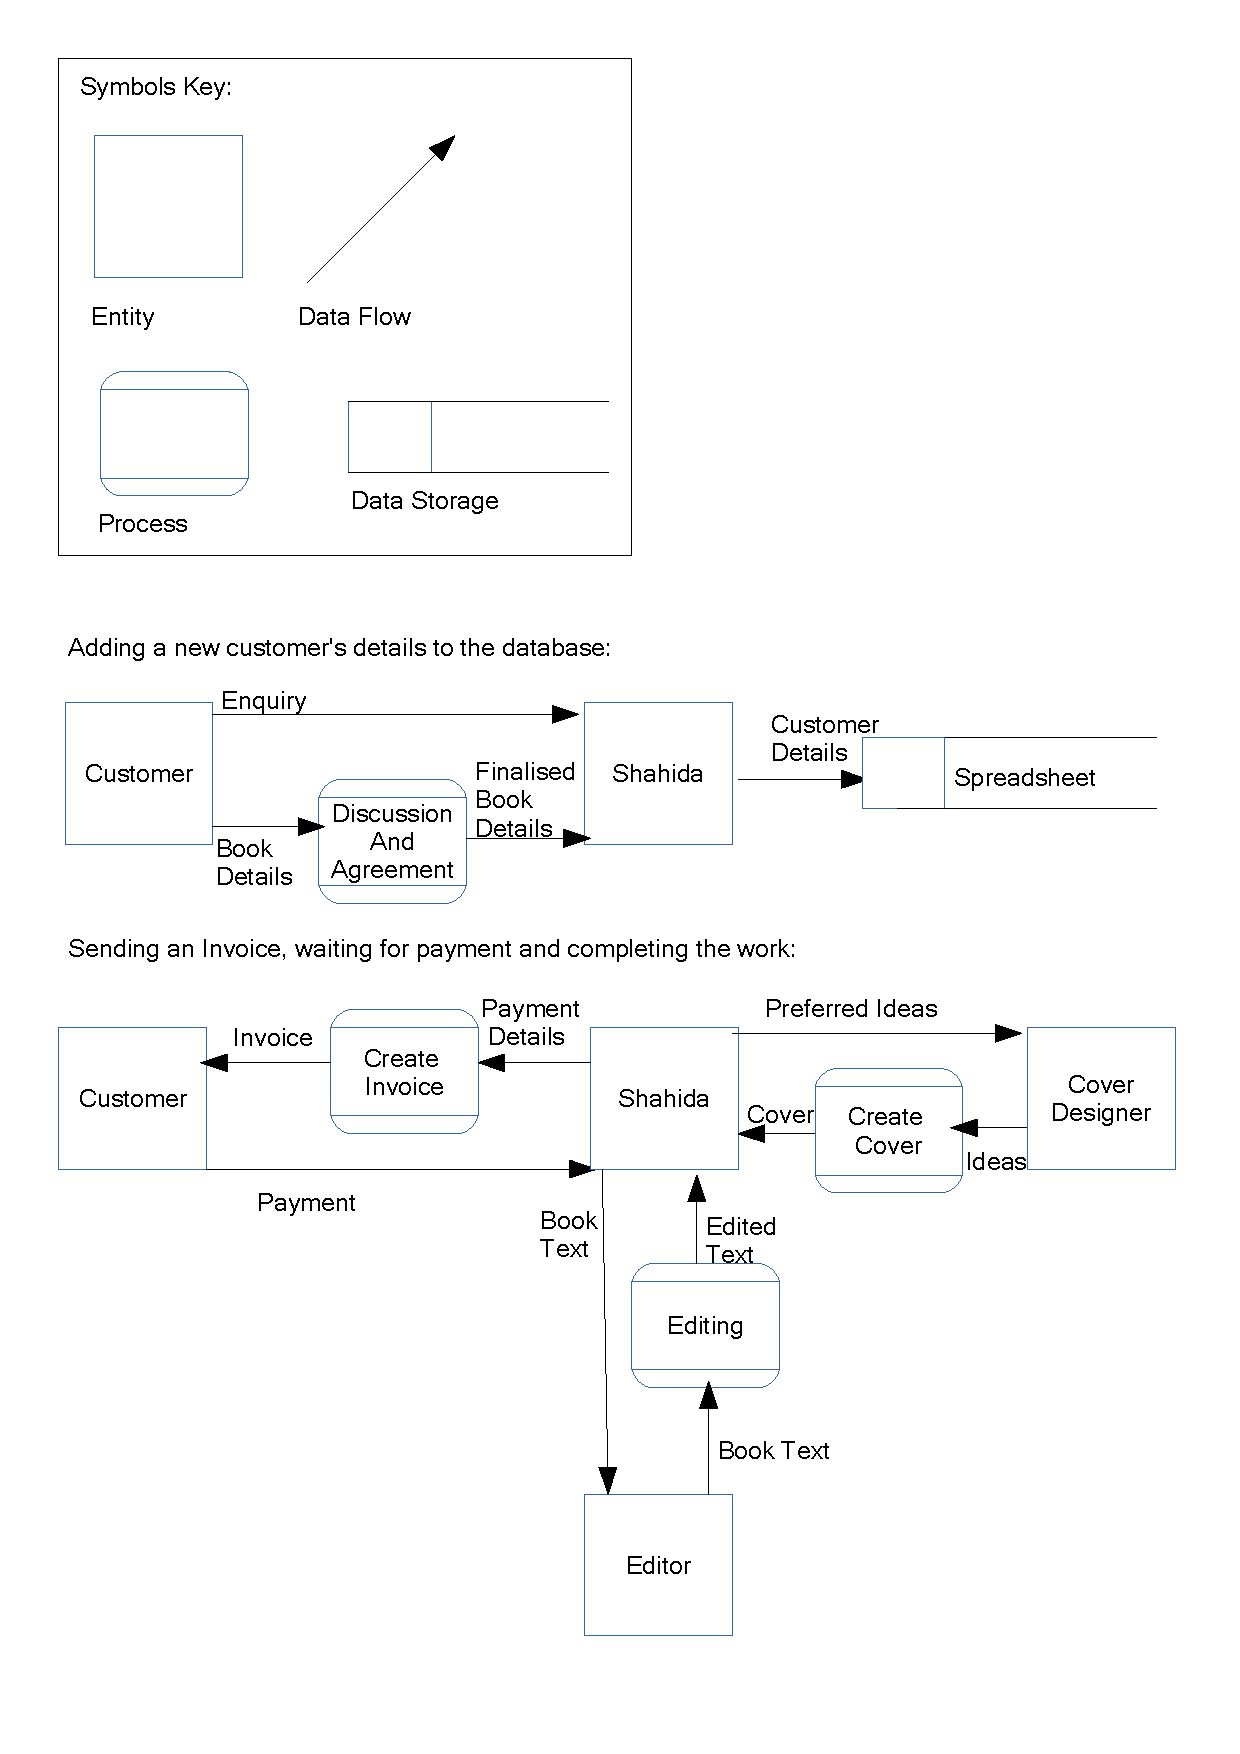
\includegraphics[width=\textwidth]{./Analysis/Data Flow Diagrams 1.pdf}
\end{figure}

\subsubsection{Input Forms, Output Forms, Report Formats}

The current system has just one input form. This is the Enquiry that is sent to the company, from an author. Also, The current system has two different output forms - The Invoice and The Royalty Statement.


The enquiry is received via email, which is sent using the company's website. The email will look like this when received:


First Name:

Last Name:

Email:

Question/Comment:



The following image is an example of the first output form, an Invoice.

\begin{figure}[H]
    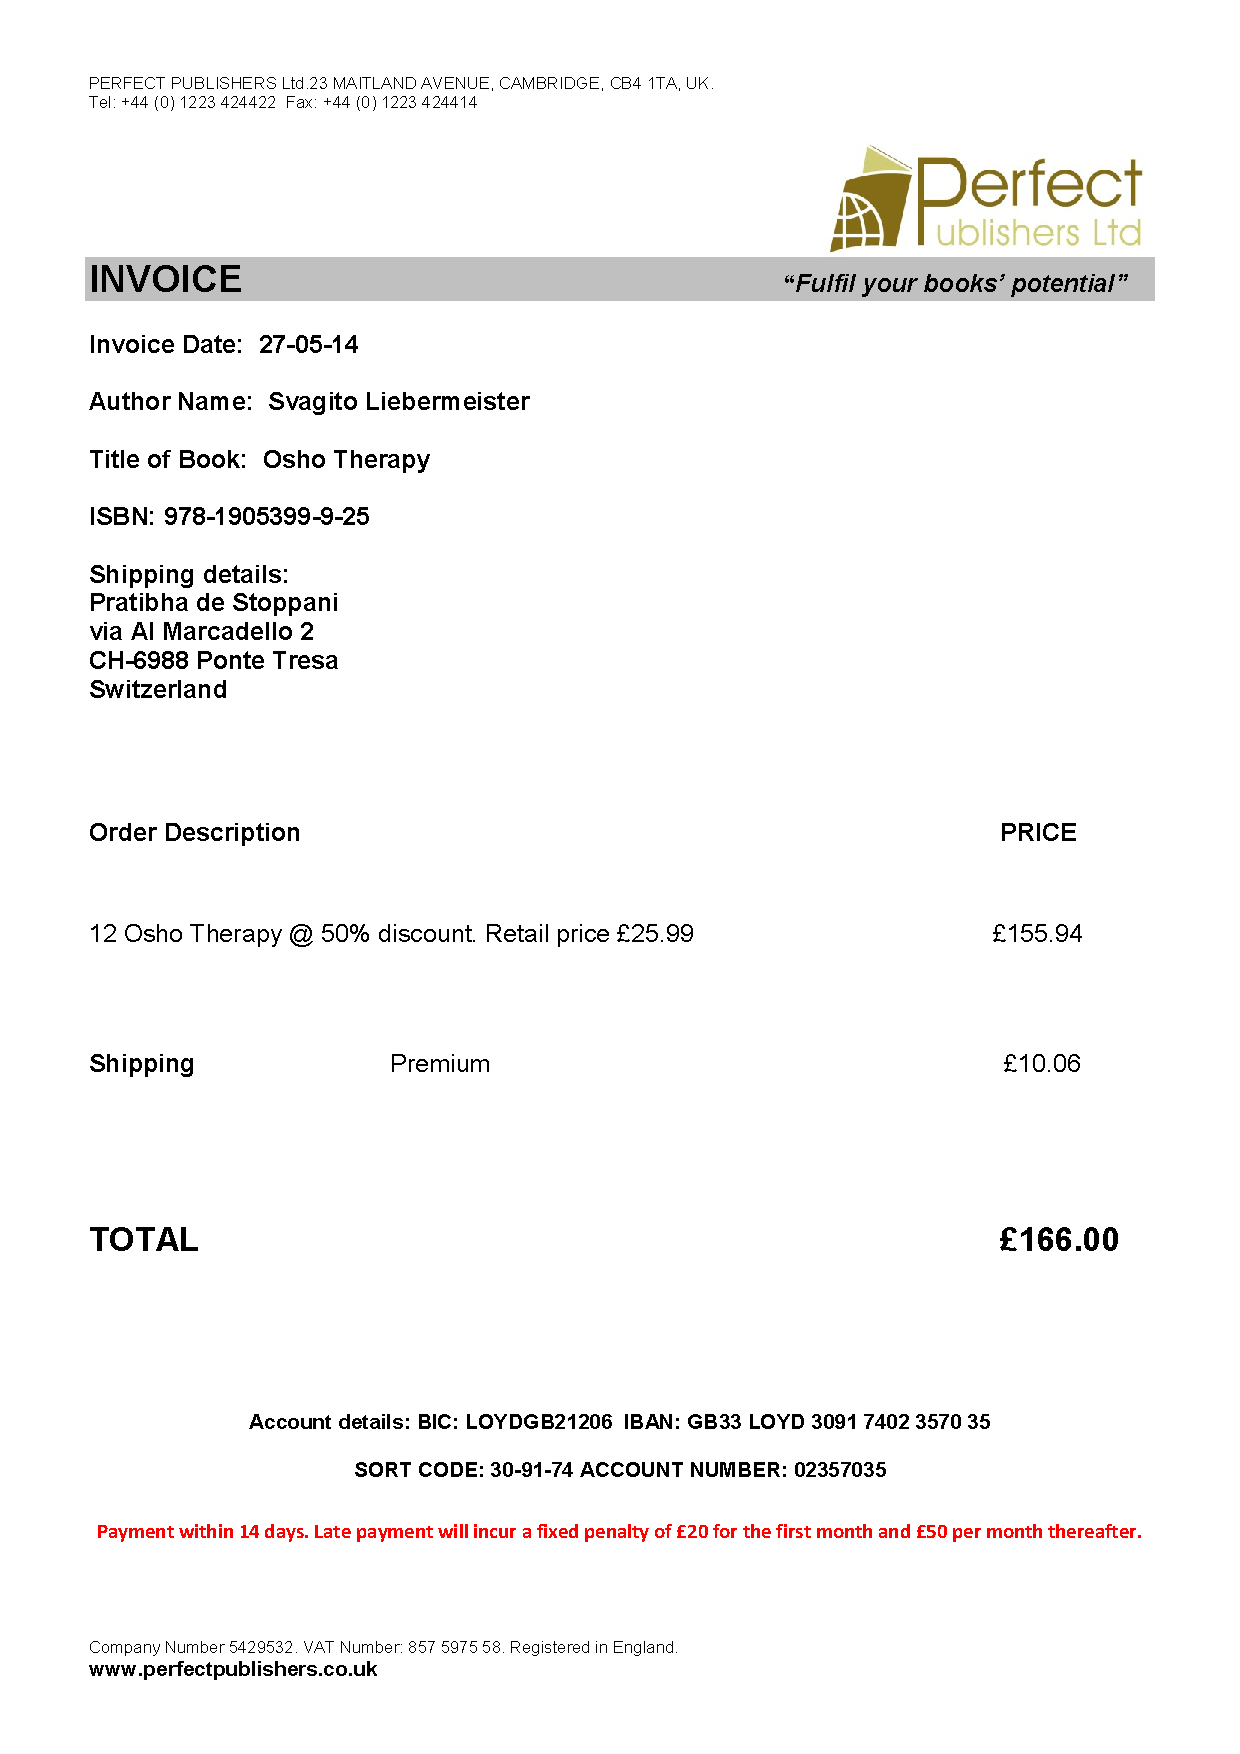
\includegraphics[width=\textwidth]{./Analysis/Invoice Example.pdf}
\end{figure}


The following image is an example of the second output form, a Royalty Statement.

\begin{figure}[H]
    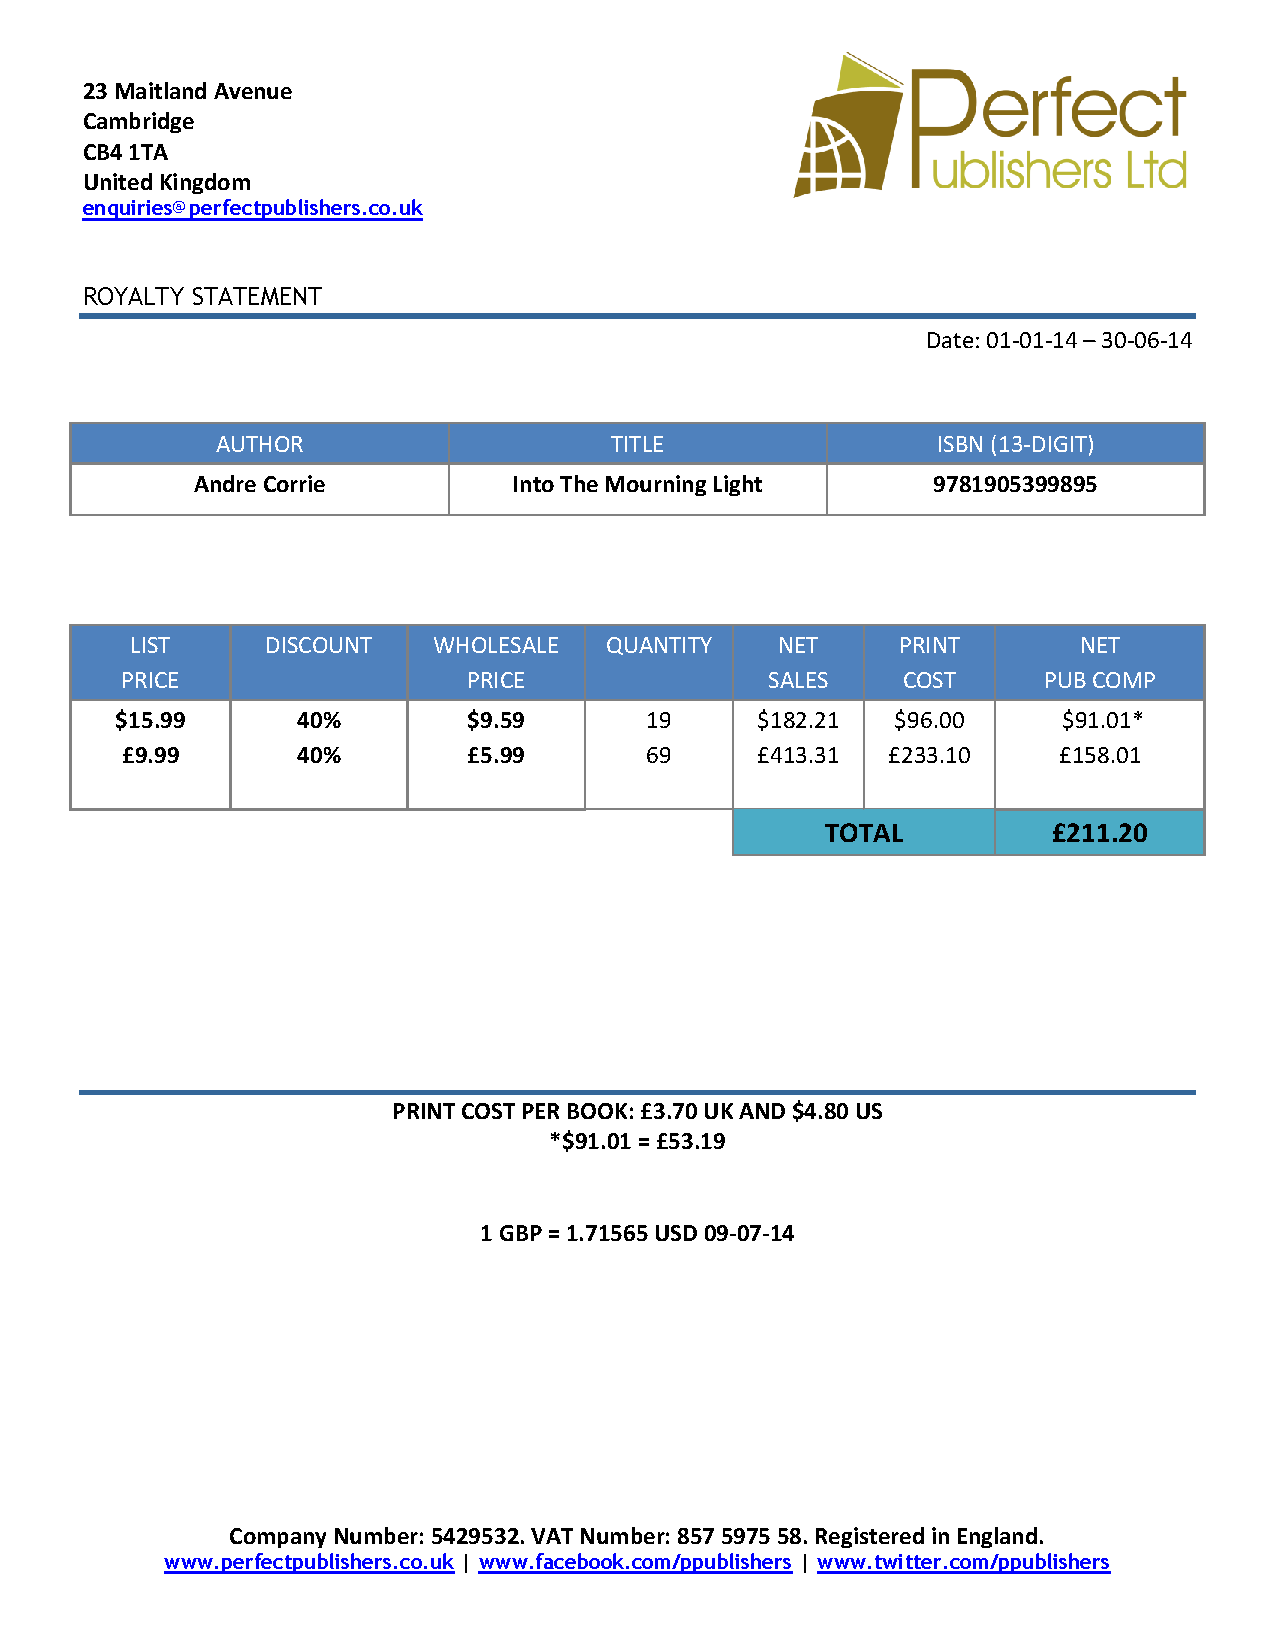
\includegraphics[width=\textwidth]{./Analysis/Royalty Statement Example.pdf}
\end{figure}

\subsection{The proposed system}

In the proposed system the Customer's information will still be received through the online form on the company's website, which Shahida receives via email. She will then enter this into the system using a new interface that will ask her for the details. This will be placed into a database. Each Customer's book will have a primary key, the ISBN number. In a seperate database, the author's details will be stored and the author will have a special ID number which is used only in the databases. Every book that is published by the same author will have an attribute which is the author's ID. The ID will just be a number. The system's interface will have a search feature, which can search for book titles, authors, and author IDs.

\subsubsection{Data sources and destinations}
\begin{center}
\begin{tabular}{|p{2.5cm}|p{3.5cm}|p{3.5cm}|p{2.5cm}|}
    \hline
    \textbf{Source} & \textbf{Data} & \textbf{Data Type} & \textbf{Destination} \\ \hline
    \pythoninline{Customer Enquiry} & \pythoninline{Forename} & \pythoninline{String} & \pythoninline{Shahida}  \\ \hline
    \pythoninline{Customer Enquiry} & \pythoninline{Surname} & \pythoninline{String} & \pythoninline{Shahida}  \\ \hline
    \pythoninline{Customer Enquiry} & \pythoninline{Email} & \pythoninline{String} & \pythoninline{Shahida}  \\ \hline
    \pythoninline{Customer} & \pythoninline{Address} & \pythoninline{String} & \pythoninline{Shahida}  \\ \hline
    \pythoninline{Customer} & \pythoninline{Postcode} & \pythoninline{String} & \pythoninline{Shahida}  \\ \hline
    \pythoninline{Customer} & \pythoninline{Phone Number} & \pythoninline{String} & \pythoninline{Shahida}  \\ \hline
    \pythoninline{Shahida} & \pythoninline{Forename} & \pythoninline{String} & \pythoninline{Database}  \\ \hline
    \pythoninline{Shahida} & \pythoninline{Surname} & \pythoninline{String} & \pythoninline{Database}  \\ \hline
    \pythoninline{Shahida} & \pythoninline{Email} & \pythoninline{String} & \pythoninline{Database}  \\ \hline
    \pythoninline{Shahida} & \pythoninline{Address} & \pythoninline{String} & \pythoninline{Database}  \\ \hline
    \pythoninline{Shahida} & \pythoninline{Postcode} & \pythoninline{String} & \pythoninline{Database}  \\ \hline
    \pythoninline{Shahida} & \pythoninline{PhoneNumber} & \pythoninline{String} & \pythoninline{Database}  \\ \hline
    \pythoninline{Database} & \pythoninline{Author ID} & \pythoninline{Integer} & \pythoninline{Shahida, Database}  \\ \hline
    \pythoninline{Shahida} & \pythoninline{Invoice} & \pythoninline{String} & \pythoninline{Customer}  \\ \hline
    \pythoninline{Customer} & \pythoninline{Payment} & \pythoninline{-} & \pythoninline{Shahida}  \\ \hline
    \pythoninline{Shahida} & \pythoninline{Cover Details} & \pythoninline{String} & \pythoninline{Cover Designer}\\ \hline
    \pythoninline{Shahida} & \pythoninline{Book} & \pythoninline{String} & \pythoninline{Editor}  \\ \hline
    \pythoninline{Editor} & \pythoninline{Completed Book} & \pythoninline{String} & \pythoninline{Shahida}  \\ \hline
    \pythoninline{Cover Designer} & \pythoninline{Completed Cover} & \pythoninline{-} & \pythoninline{Shahida} \\ \hline
    \hline
\end{tabular}
\end{center}

\subsubsection{Data flow diagram}

\begin{figure}[H]
    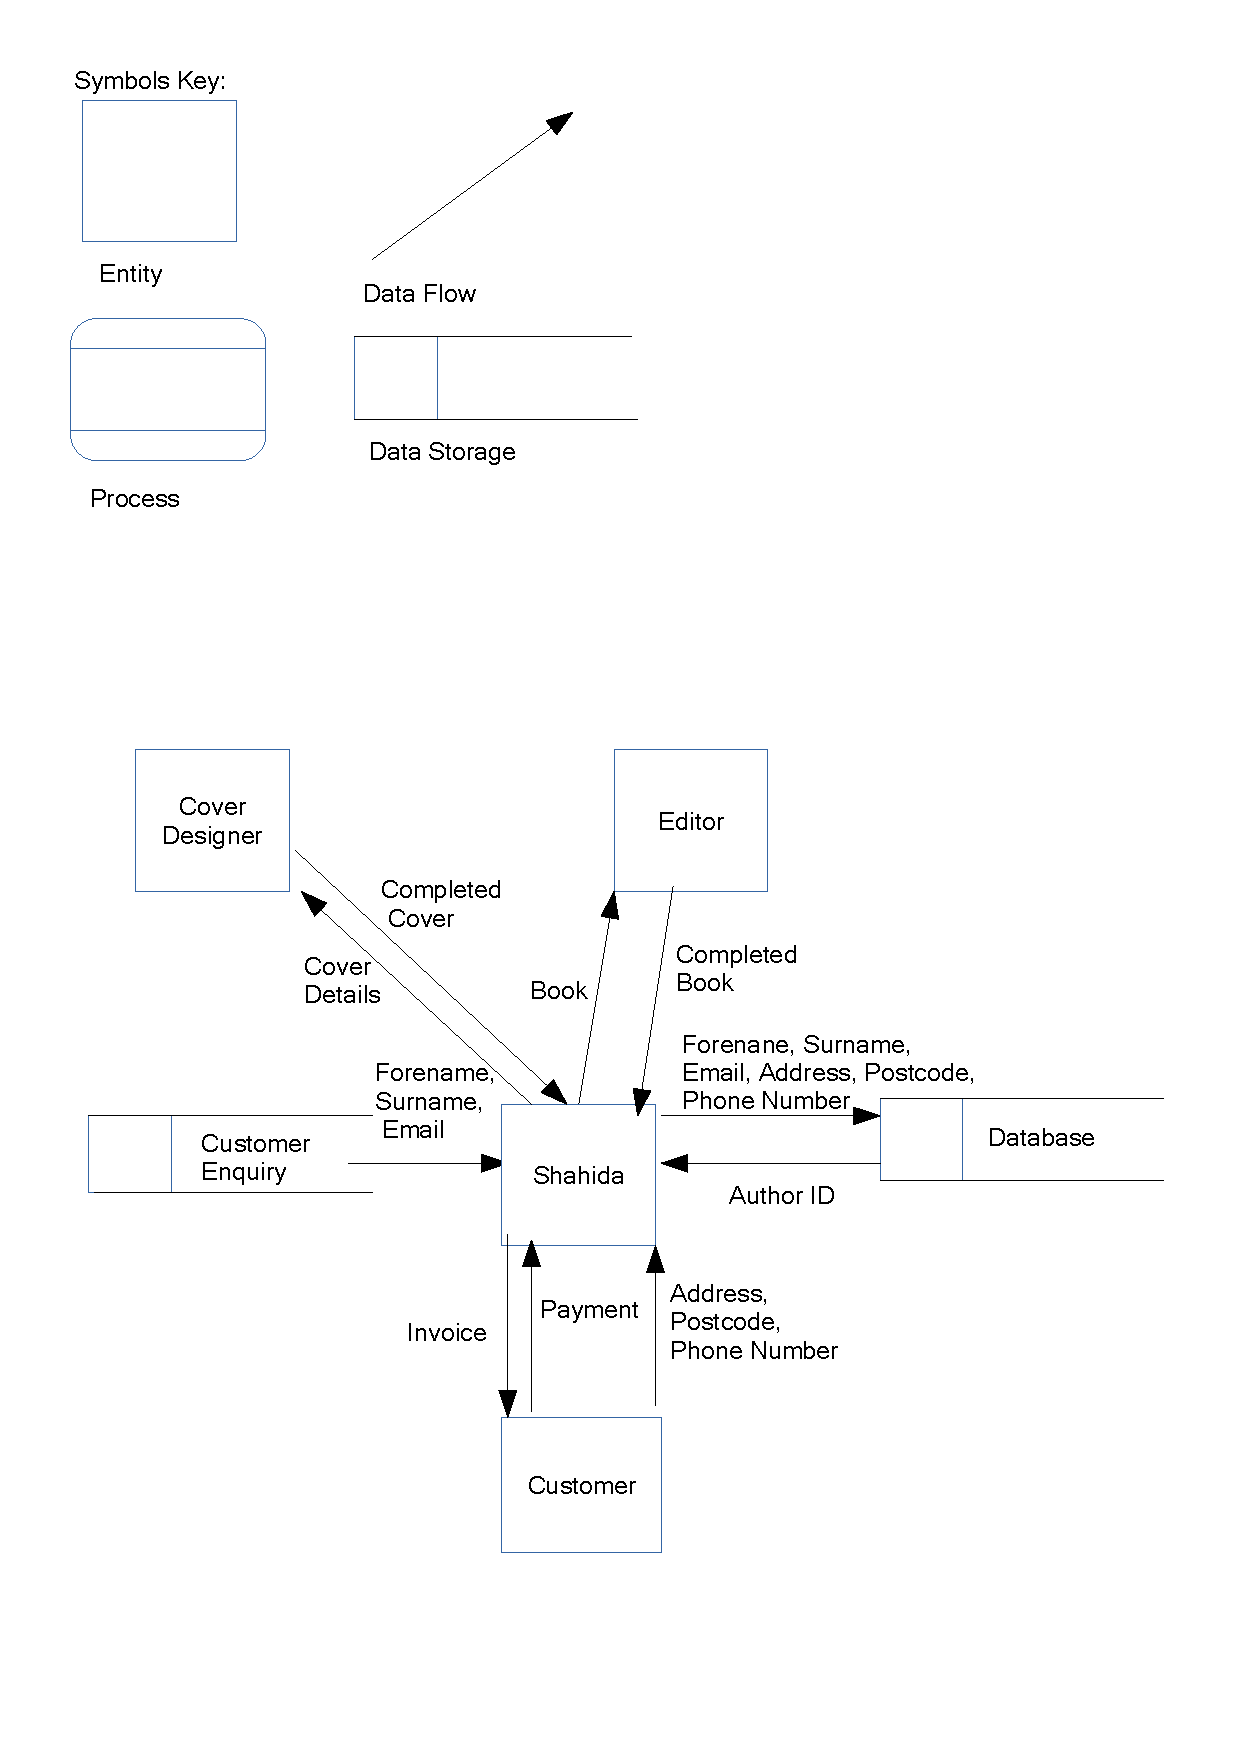
\includegraphics[width=\textwidth]{./Analysis/Data Flow Diagrams 2.pdf}
\end{figure}

\subsubsection{Data dictionary}

\begin{center}
\begin{tabular}{|p{2.5cm}|p{2.5cm}|p{2.5cm}|p{2.5cm}|p{2.5cm}|p{2.5cm}|}
    \hline
    \textbf{Name} & \textbf{Data Type} & \textbf{Length} & \textbf{Validation} & \textbf{Example Data} \\ \hline
    \pythoninline{FirstName} & \pythoninline{String} & \pythoninline{2-20 Characters} & \pythoninline{Length} & \pythoninline{Jo}  \\ \hline
    \pythoninline{LastName} & \pythoninline{String} & \pythoninline{2-20 Characters} & \pythoninline{Length} & \pythoninline{Williamson}  \\ \hline
    \pythoninline{Email} & \pythoninline{String} & \pythoninline{7-30 Characters} & \pythoninline{Length} & \pythoninline{mail@example.com}  \\ \hline
    \pythoninline{PhoneNumber} & \pythoninline{String} & \pythoninline{9-15 Characters} & \pythoninline{Format} & \pythoninline{07123456789}  \\ \hline
    \pythoninline{Address} & \pythoninline{String} & \pythoninline{5-30 Characters} & \pythoninline{Length} & \pythoninline{Example Road}  \\ \hline
    \pythoninline{Postcode} & \pythoninline{String} & \pythoninline{7 Characters} & \pythoninline{Format} & \pythoninline{AB1 2CD}  \\ \hline
    \pythoninline{Author ID} & \pythoninline{Integer} & \pythoninline{1-255} & \pythoninline{Range} & \pythoninline{17}  \\ \hline
    \pythoninline{BookTitle} & \pythoninline{String} & \pythoninline{1-60 Characters} & \pythoninline{Length} & \pythoninline{The Hobbit}  \\ \hline
    \pythoninline{NoOfPages} & \pythoninline{Integer} & \pythoninline{1-1027} & \pythoninline{Range} & \pythoninline{395}  \\ \hline
    \pythoninline{SizeLarge} & \pythoninline{Boolean} & \pythoninline{-} & \pythoninline{Existence} & \pythoninline{False}  \\ \hline
    \pythoninline{SizeSmall} & \pythoninline{Boolean} & \pythoninline{-} & \pythoninline{Existence} & \pythoninline{True}  \\ \hline
    \pythoninline{Hardback} & \pythoninline{Boolean} & \pythoninline{-} & \pythoninline{Existence} & \pythoninline{False}  \\ \hline
    \pythoninline{Paperback} & \pythoninline{Boolean} & \pythoninline{-} & \pythoninline{Existence} & \pythoninline{True}\\ \hline
    \pythoninline{Mat} & \pythoninline{Boolean} & \pythoninline{-} & \pythoninline{Existence} & \pythoninline{False}  \\ \hline
    \pythoninline{Gloss} & \pythoninline{Boolean} & \pythoninline{-} & \pythoninline{Existence} & \pythoninline{True}  \\ \hline
    \pythoninline{CremePaper} & \pythoninline{Boolean} & \pythoninline{-} & \pythoninline{Existence} & \pythoninline{False}  \\ \hline
    \pythoninline{WhitePaper} & \pythoninline{Boolean} & \pythoninline{-} & \pythoninline{Existence} & \pythoninline{True}\\ \hline
    \pythoninline{Font} & \pythoninline{String} & \pythoninline{-} & \pythoninline{Existence} & \pythoninline{Arial}  \\ \hline
    \pythoninline{FontSize} & \pythoninline{Floating point} & \pythoninline{1-5 Characters} & \pythoninline{} & \pythoninline{12.5}  \\ \hline
    \hline
\end{tabular}
\end{center}

\subsubsection{Volumetrics}

I have chosen to use a size of 100 different customer records. This is because the company rarely have more than 20 enquiries in a year. This would be a suitable size as it will last a few years before it may require resizing, which can be conducted at a later date when necessary.

\section{Objectives}

\subsection{General Objectives}

The general objectives are:
\begin{itemize}
    \item Organised layout for the database.
    \item Prevention of unnecessary duplication of data.
    \item Simple interface for entering data.
    \item Search function to find a specific customer in the database
    \item Ability to edit existing data easily
    \item Ability to calculate royalties using given data
\end{itemize}

\subsection{Specific Objectives}

Organising a layout for the database:

\begin{itemize}
    \item Be able to sort by date (ascending and descending)
    \item Clear tables and fields for each entity and attribute
\end{itemize}


Preventing Duplication:

\begin{itemize}
    \item Checks to see if the data already exists
    \item Use of Author ID to ensure it will only be entered once
\end{itemize}


Simple interface for entering data:

\begin{itemize}
    \item As little amount of boxes as possible
    \item Clearly label entry boxes
\end{itemize}


Search function and editing data:

\begin{itemize}
    \item Data can be found using the Author ID, Author Name, or Book Title
    \item Can be edited upon finding the desired data
\end{itemize}


Calculating royalties:

\begin{itemize}
    \item Receives inputs from user (print cost, wholesale price and quantity sold)
    \item Uses inputs to calculate the royalties
\end{itemize}

\subsection{Core Objectives}

\begin{itemize}
    \item Organising the data using certain attributes
    \item Calculating royalties
    \item Preventing Duplication
\end{itemize}

\subsection{Other Objectives}

\begin{itemize}
    \item Searching for data using attributes
    \item Editing data in the database
\end{itemize}

\section{ER Diagrams and Descriptions}

\subsection{ER Diagram}
%

\subsection{Entity Descriptions}
%
\section{Object Analysis}

\subsection{Object Listing}

\begin{itemize}
    \item Customer
    \item Book
    \item Enquiry
    \item Shahida
\end{itemize}

\subsection{Relationship diagrams}
%
\subsection{Class definitions}
%
\section{Other Abstractions and Graphs}

\section{Constraints}

\subsection{Hardware}
Shahida uses her laptop to run the company from home. The new system will need to be able to run on this machine.

Computer Specifications:

\begin{itemize}
    \item 15.6” Display
    \item AMD Quad-Core A4-5000M APU (1.5GHz, 2MB cache)
    \item 4 GB DDR3 RAM
    \item 750 GB HDD, 5400 rpm
    \item AMD Radeon HD 8330 Graphics Card
\end{itemize}

The proposed system will have no problem with running on this machine, as it uses a small amount of CPU usage. A constraint would be the size of the screen. This is because the system will need to be based around the screen size of her laptop. As her laptop is portable, portability is not a constraint.

\subsection{Software}

Shahida would prefer that the system will run on Windows 7, as she uses this operating system for her laptop. Changing the operating system will cause difficulties, meaning it is best for the system to run on Windows 7, suiting her needs.

\subsection{Time}

Shahida does not need this system to be built quickly, but she would like it to be complete as soon as reasonably possible. Otherwise, the only time restriction for this project is , which has been set by my teacher.

\subsection{User Knowledge}

Having worked in the publishing industry beforehand, being an author has also given Shahida the knowledge of how to run her current company. 

\subsection{Access restrictions}

Shahida will be the only person who will have full access to all the data in the proposed system, and she will be the only one who can access it. This can be password protected for security reasons, meaning that only she can gain access to the database. The database will comply to the Data Protection Act 1998, as the company already does so with their current system.

\section{Limitations}

\subsection{Areas which will not be included in computerisation}
Generally, all actions require the use of a computer in the company. However, rarely, a customer does call Shahida about an enquiry, as this customer may not be so computer literate. In this case, Shahida will note down the details of the enquiry, and will enter it into the database.
\subsection{Areas considered for future computerisation}

The database could be used online, so that the authors can use their Author ID to log in and see just their details on the database. This would mean that the customers would not have to contact Shahida to receive the data held about them, as they can see the data by theirselves.

\section{Solutions}

\subsection{Alternative solutions}
\begin{center}
\begin{tabular}{|p{2.5cm}|p{3.5cm}|p{3.5cm}|}
    \hline
    \textbf{Solution} & \textbf{Advantages} & \textbf{Disadvantages} \\ \hline
    \pythoninline{Re-organisation of the current spreadsheet} & \pythoninline{No changes to current operating system and software} & \pythoninline{Current problems will still occur, Difficult to keep organised} & \pythoninline{Shahida}  \\ \hline
    \pythoninline{Python Desktop Application with GUI} & \pythoninline{User Friendly, Clear and easy to interpret} & \pythoninline{Takes up more memory, Takes longer to create the application} & \pythoninline{Shahida}  \\ \hline
    \pythoninline{Filing system} & \pythoninline{No electronics needed} & \pythoninline{More problems may be encountered than the current system, Lots of physical space is required} & \pythoninline{Shahida}  \\ \hline
    \hline
\end{tabular}
\subsection{Justification of chosen solution}
I have chosen to use the Python Desktop Application with GUI as my solution. This is because:

\begin{itemize}
    \item I am already familiar with the Python Programming Language.
    \item This will keep the system using computers and software, meaning there will not be a drastic change.
    \item Using the application will take less time than manually entering everything into a spreadsheet, and less time than writing details down on paper.
\end{itemize}
